\subsection{Systemanalyse und -entwurf}

Aufbauend auf die Anforderung, einen Prototypen mit den Technologien der SAP Leonardo IoT Foundation zu entwickeln, wird in diesem Kapitel die zugrundeliegende Systemarchitektur untersucht. Dabei erfüllt die Analyse mehrere Zwecke. Zum einen wird die Forschungsfrage FF-1.2 (s. \ref{problemstellung}), welche Möglichkeiten zur intelligenten Vernetzung die Architektur bietet, beantwortet. An die Beantwortung dieser Frage knüpft sich die Prüfung der Kompatibilität der Zielarchitektur mit der \ac{rami}. In der Anforderungsanalyse wurde hauptsächlich die Anwendung des cloud-basierten Ansatzes als Lösung (s. \ref{technischeraufbau}) spezifiziert. Aus diesem Grund wird auf Grundlage der Analyse die angepasste Architektur des Zielsystems als Lösung für den technischen Aufbau entworfen.

\subsubsection{Systemarchitektur}

Wie in Abschnitt \ref{leo} beschrieben, bietet die SAP Leonardo IoT Foundation zahlreiche Dienste zur Integration von physischen Geräten in die SAP Cloud Platform und somit in die Geschäftswelt. Somit entstehen \ac{cpss}, welche im Rahmen eines \ac{iot}-Projektes typischerweise drei Phasen durchlaufen: \textit{Datentransport, Datenhaltung und Analyse} (s. Abschnitt \ref{technologien}). Wie die Architektur der SAP Leonardo IoT Foundation diesen Integrationsprozess bewerkstelligt, ist in Abbildung \ref{saparch} zu sehen. Die realen Geräte senden ihre Daten über \textit{Gateways} mit verschiedenen Netzwerkprotokollen an die \textit{SAP Cloud Platform Internet of Things Services} (1). Dort werden sie in einer PostgreSQL Datenbank gehalten \citep{Acharya2019}. Der Zugriff auf die Daten der \ac{cpss} erfolgt im Rahmen einer service-orientierten Architektur (SOA) über verschiedene \ac{api}. Um die Geräte in eine IoT-Anwendung zu integrieren, werden sie via \textit{Message Processing} and das \textit{IoT Application Enablement} gesendet (2). Dort können digitale Zwillinge erstellt, funktionalisiert und analysiert werden. Für die Anwendungsentwicklung werden die Daten per OData- oder REST-Schnittstellen von der Cloud Foundry Umgebung an die WebIDE in der Neo Umgebung übergeben (3). Anschließend wird die Anwendung in die Cloud Foundry deployed. Die einzelnen Komponenten und Konzepte werden im Folgenden näher im Detail erläutert.

\begin{figure}[ht!]
  \centering
  \noindent\makebox[\textwidth]{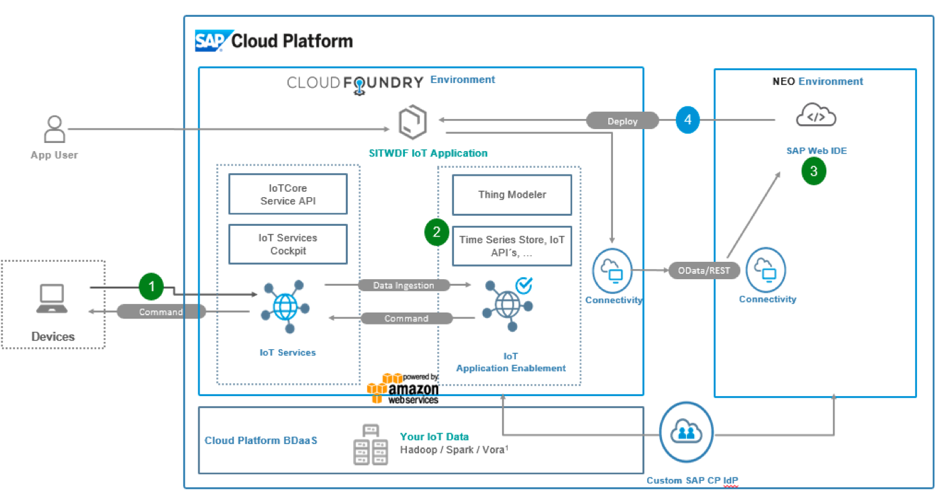
\includegraphics[width=\paperwidth]{sap_architecture.png}}
  \caption[Architektur von SAP]{Architektur von SAP \citep{Ganz2019}}
  \label{saparch}
\end{figure}

\newpage
\subsubsection{Datentransport: Internet of Things Gateway}



  Der erste Schritt von einem realen physischen Ding zu einem \ac{cpss} ist der Datentransport zu einem Datenobjekt im Netz (s. \ref{technologien}). Bezogen auf \ac{rami} und das Konzept der \acf{i40} ist dies der Prozess der Integration und Kommunikation. Das reale Objekt wird an ihre Verwaltungsschale angebunden, um virtuell repräsentiert werden zu können. Die Architektur von SAP bietet für diesen Vorgang zwei Möglichkeiten. Entweder den direkten Transport der Daten in die Cloud über die \textit{Gateway Cloud} oder über die \textit{Internet of Things Edge Platform}. Neben dem senden von Messwerten in die Cloud können außerdem aus der Cloud heraus Befehle an das Gerät gesendet werden. Welche Variante auszuwählen ist, hängt von individuellen Anwendungsfällen und benötigten Protokollen ab. Die \textit{Gateway Cloud} wird in dem \textit{SCP Internet of Things Service} standardmäßig für MQTT und REST mitgeliefert.
  \begin{wraptable}[16]{r}{0.4\textwidth}
    \caption{Gateway-Protokolle}\label{gateway}
    \begin{tabular}{ccc}\\\toprule
    Protokoll & Cloud & Edge \\\midrule
    MQTT &x & x\\  \midrule
    HTTP (REST) & x & x\\  \midrule
    CoAP& & x\\  \midrule
    File &  & x\\  \midrule
    Modbus & & x\\  \midrule
    OPC UA & & x\\  \midrule
    SigFox & & x\\  \midrule
    SNMP & & x\\  \bottomrule
    \end{tabular}
    \label{protocol}
  \end{wraptable}
  \newline
  Die \textit{Internet of Things Edge Platform} wird von den Entwicklern lokal auf dem Gerät nach dem ausgewählten Kommunikationsprotokoll (s. Tabelle \ref{protocol}) selbst konfiguriert. Sie dient dazu, Messwerte von Geräten mit mangelnder Internetverbindung zu verarbeiten und bei verfügbarerer Verbindung an die Cloud zu senden. In beiden Fällen werden die Nachrichten mit den Messwerten im \ac{json}- oder im \ac{protobuf}-Format mit POST-Anfragen an die API-Endpunkte der registrierten Geräte gesendet \citep{SAP2020}. Das Registrieren der Geräte wird im nächsten Kapitel näher behandelt. SAP bietet außerdem die Möglichkeit, das \textit{Internet of Things Service} mit dem \textit{Internet of Things Edge Platform SDK} zu erweitern. Das SDK bietet Tools auf Eclipse, das Gateway mit \textit{Interceptors} zu erweitern. Die Messwerte können vor dem Senden an die Cloud vom Gateway abgefangen, modiziert oder gefiltert werden.

  \begin{lstlisting} [label=lst:endpunkt, caption=API-Endpunkte der Gateways]
    // Endpunkt der Gateway Cloud
    https://<HOST_NAME>:443/iot/gateway/rest/measures/<deviceAlternateId>
    // Endpunkt des Edge Gateways
    https://<IOT_GATEWAY_IP>:8699/measures/<deviceAlternateId>
  \end{lstlisting}

  %------------------------------------------


\subsubsection{Datenhaltung: SCP Internet of Things Service} \label{iotcp}

Wie in Listing \ref{lst:endpunkt} zu sehen ist, haben die Gateways, welche die Daten der Geräte an die Cloud übermitteln, eine \textit{deviceAlternateId} zum Ziel. Damit die Daten in der Cloud ankommen können,müssen die Geräte und Sensoren für die Messwerte im \textit{Internet of Things Service} der SAP Cloud Platform registriert werden. Für diesen Zweck liefert SAP ein Datenmodell für die Geräte, nach dem eine Entität des Geräts erstellt werden muss (s. Abbildung \ref{fig:devicemodel}). Nach dem Modell muss ein Gerät mindestens aus einem Sensor bestehen und eindeutig einem Gateway zugeordnet sein. Die Sensoren sind immer Instanzen von bestimmten Sensortypen, denen Fähigkeiten und Eigenschaften zugeordnet werden.
Für die Registrierung bietet das System zwei Möglichkeiten. Man es kann entweder über die grafische Benutzeroberfläch des \textit{IoT Services Cockpit} durch das Ausfüllen von Formularen erstellen oder über die \textit{IoT Core Service API} (s. Abbildung \ref{saparch}). In beiden Fällen werden POST-Anfragen im \ac{json}-Format an den API-Endpunkt des Tenants im \textit{Internet of Things Service} gesendet. Für diesen Zweck stellt SAP eine Sammlung von \textit{Device Management API} zur Verfügung. Nachdem die Geräte registiert wurden, kann die SAP Cloud Platform das Datenobjekt des \acf{cpss}halten. Somit befindet sich das physische Ding in der Informationsschicht nach \ac{rami}.

\begin{figure}[ht!]
  \centering
  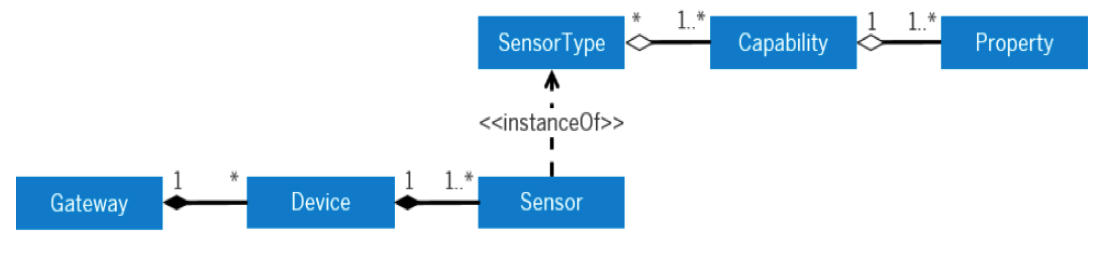
\includegraphics[width=1.0\linewidth]{pictures/device_model}
  \caption[Gerätemodell]{Gerätemodell}
  \label{fig:devicemodel}
\end{figure}

\noindent Genau so wie das Erstellen von Geräten über APIs, kann auf Messwerte und Eigenschaften der Geräte über GET-Anfragen an die API-Endpunkte zugriffen werden. Der Zugriff auf die Daten nennt sich in diesem  Kontext \textit{Message Processing} und kann über die von SAP zur Verfügung gestellte Sammlung von \textit{Message Processing API} konfiguriert und abgerufen werden. Diese Schnittstellen sind vor allem hinsichtlich der Einbindung der Daten in externe Dienste und Anwendungen von großer Relevanz. Je nach Bedarf und Anwendungsfall können unterschiedliche Dienste konfiguriert werden \citep{SAP2020}:
\begin{itemize}
  \item \textit{SAP Leonardo IoT Integration} für den Datentransfer an SAP Leonardo IoT
  \item \textit{SQL} für den Fall, dass die Gerätedaten in einer externen DB gespeichert werden sollen
  \item \textit{Kafka} z.B. für Big-Data Dienste
  \item \textit{HTTP}, um einen eigenen API-Endpunkt zu nutzen
\end{itemize}

\subsubsection{Analyse: SAP Leonardo IoT}

Über den Message Processing Service \textit{SAP Leonardo IoT Integration} werden die Daten der Geräte an SAP Leonardo IoT übergeben. Laut SAP bietet Leonardo IoT \glqq alle notwendigen Funktionen zum Einrichten von Thing- und Geschäftspartnerstrukturen als Repräsentation der Realen Welt\grqq{} \citep[S. 11]{SAP2019} Aber eigetnlich sind das Microservices zum Erstellen digitaler Zwillinge, Analysedaten und WebApps. Mithilfe der Microservices und Werkzeuge können einfach IoT-Anwendungen erstellt werden. Grundlage dafür ist zunächst der \textit{Thing Modeler}, mit dem digitale Zwillinge der registrierten Geräte erstellt werden.
Neue Architektur Screenshot rein
API Aggregatiwn blllla
Für die Integration der Geräte in Anwendungen werden hier digitale Zwllinge erstellt
Thing Modeler und freestyle IoT Applications

\subsubsection{Destinations}
Destinations: Warum braucht man Destinations und welche man benötigt (SNS),  wenn man kommunizieren will mit
Externe Services wie AWS SNS
Interne Kommunikation der SCP CF und NEO
Communication zwischen Cloud Services AWS SNS und SAP Leonardo

% Sicherheir
\subsubsection{Sicherheit}
Security Documentation
OAuth, SSL/TLS, SAML 2.0: erklären, was SAP und AWS auch eventuell haben
Device certificate für Sichere Verbindung via REST und MQTT
\subsubsection{Kompatibiliät mit Referenzarchitektur}

\begin{figure}[H]
  \centering
  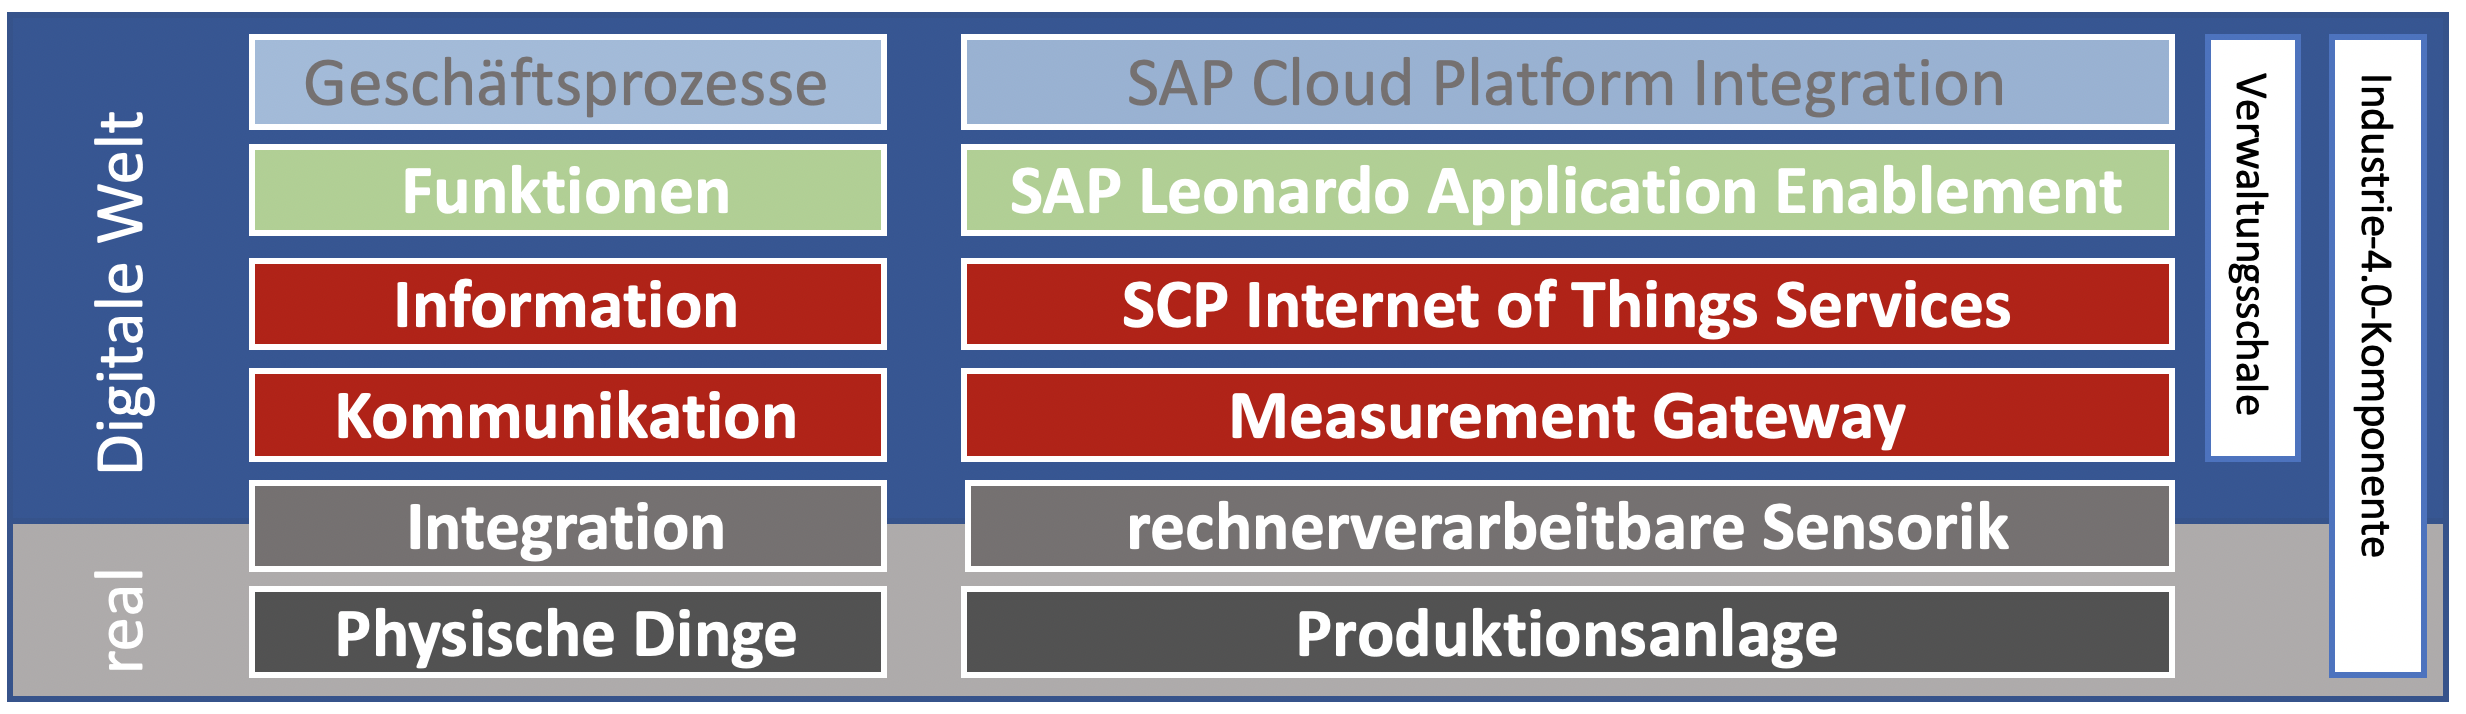
\includegraphics[width=1.0\linewidth]{pictures/rami_custom1}
  \caption[Referenz zu den Schichten der RAMI 4.0]{Referenz zu den Schichten der RAMI 4.0}
  \label{ramicustom}
\end{figure}

\begin{figure}[h]
  \centering
  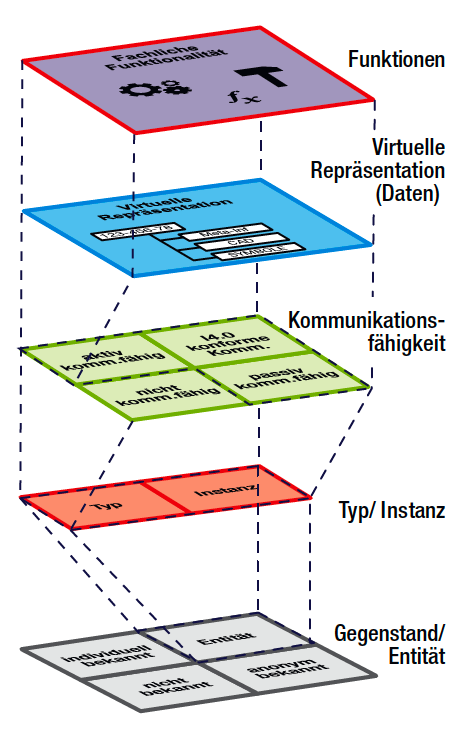
\includegraphics[width=0.5\linewidth]{Ebenen_I40_Kompo.png}
  \caption[Ebenen der Industrie-4.0-Komponente]{Ebenen der Industrie-4.0-Komponente \citep[S. 52]{BITKOM2015}}
  \label{ebenen_i40}
\end{figure}

\subsubsection{Systementwurf gemäß Architekturkonzept}

eigene Architektur aufmalen

